\cleardoublepage%
\chapter{\label{chap:res}Results and Discussion}%

%This is where you present your findings. As much as possible, structure your results along the lines of your research questions. Start with the simplest results first and proceed to more complex ones. Tables and Figures should be clear enough that they need little explanation: do not simply re-write the numbers as text to fill space. Rather, highlight trends, outliers, or gaps. 

\section{\label{sec:res_networking}Networking}%should this be in firmware?

Refer to research question 1

\subsection{\label{sec:res_logic}Concept, Structure and Logic}

As outlined in Section \ref{sec:methods_net_des} and Section \ref{sec:methods_net_dev}, the networking was designed and developed in two parts, the base networking.py library and using the interfaces of the base networking as a base, the more specific ssp\_networking.py. \\

The base networking.py library is designed to be a general purpose library that builds on ESP-NOW and adds some basic structure and functionality. This base networking introduces address book logic that bypasses ESP-NOW's 20 peer limit, allowing transmission to a theoretically unlimited number of peers at the expense of efficiency. It also introduces the basic message structure, including different message types (cmd, inf, ack) and different subtypes (cmd: ping, echo, boop; inf: msg, data; ack: pong, echo, boop). The library also includes logic to send data larger than $241\ bytes$, the maximum payload allowed using the message structure defined in Section \ref{sec:rev_net}, increasing it to a theoretical limit of $60'928\ bytes$. However, in reality the message limit is lower, with the maximum amount successfully transmitted at about 30 kB due to the memory limitations of the MicroPython firmware running on the ESP32C3. Also, sending large messages in chunks runs the risk of some chunks being lost due to packet loss (see Section \ref{sec:res_rssi}), especially over long distances, resulting in the entire message being dropped. While there is a provision in the code to remedy this by storing all parts of a long message in a buffer, and if the receiving device is missing one or more parts of a multi-part message after some time, sending a message requesting the missing parts, this has been disabled for memory optimisation. 
The network design also includes various interfaces for customisation and the addition of additional custom commands, message types and handling logic, including custom IRQ messages. \\

Building on top of these interfaces of the base networking library, the SSP networking library introduces many additional smart module specific commands, handlers and message types, which especially ??????



, which introduces some basic message structure, shown in Figure \ref{fig:net_net_structure} and 

The specific structure of the code of the two libraries and all its commands is shown in Figure \ref{fig:net_code_structure}




Give a quick overview of the networking structure. 

Overview of networking, recall design requirements and guiding principles.

\begin{figure}[H]
    \centering
    
\includegraphics[width=.5\linewidth]{overleaf/images/placeholder.png}
    \vspace{\ftspace}
    \caption{Networking overview}
    \label{fig:Networking overview}
\end{figure}

To ammend this, 
While the structure exists for a recipient to send confirmations, nothing is done with this information so far, though users could decide to build their own handshake logic on top of our networking structure and use this, the necessary ground work is already in place.

The code is furthermore following the style Guide for Python Code based Python Enhancement Proposal 8. \citep{rossum_python_2001}

\subsection{\label{sec:res_range}Range Test}

As outlined in Section \ref{sec:methods_test_range}, the original range test was conducted using the boop-o-meter program on a street in front of the CEEO offices. The maximum range at which some messages were still being received by each of the two modules was approximately 242 meters, as shown in Figure \ref{sec:res_range}.

\begin{figure}[H]
    \centering
    \includegraphics[width=\linewidth]{overleaf/images/range.png}
    \vspace{\ftspace}
    \caption{Approximate Range Test on Boston Avenue, MA}
    \label{fig:range}
\end{figure}


\subsection{\label{sec:res_rssi}Response Time, RSSI and Packet Loss Rate by Range}

Also include results for experiments for range, rssi and latency.

\begin{figure}[H]
    \centering
    
\includegraphics[width=.5\linewidth]{overleaf/images/placeholder.png}
    \vspace{\ftspace}
    \caption{Ping figure}
    \label{fig:ping}
\end{figure}

\begin{figure}[H]
    \centering
    
\includegraphics[width=.5\linewidth]{overleaf/images/placeholder.png}
    \vspace{\ftspace}
    \caption{RSSI figure}
    \label{fig:rssi}
\end{figure}

\begin{table}[H]
    \centering
    \begin{tabular}{|c|c|l|l|c|c|c|c|c|}
    \hline
        Range & Packet Loss & \multicolumn{2}{l|}{Measurement} & \multicolumn{5}{c|}{Values} \\\hline
        [meters] & [\%] & \multicolumn{2}{l|}{} & mean & std & min & max & median \\\hline\hline
        \multirow{3}{*}{0 m} & \multirow{1}{*}{0} & RSSI 1 & [asu] & -6.05 & 1.14 & -12 & -5 & -6 \\\cline{2-9}\cline{2-9}
        %&& Time 1 &  &  &  &  &  \\\cline{2-9}\cline{2-9}
        & \multirow{2}{*}{0} & RSSI 2 & [asu] & -5.44 & 0.67 & -8 & -5 & -5 \\\cline{3-9}
        %&& Time 2 &  &  &  &  &  \\\cline{3-9}
        && Ping & [ms] & 20.57 & 0.61 & 19 & 23 & 20 \\\hline\hline
        \multirow{3}{*}{0.1 m} & \multirow{1}{*}{0} & RSSI 1 & [asu] & -15.5 & 0.59 & -17 & -15 & -15 \\\cline{2-9}\cline{2-9}
        %&& Time 1 &  &  &  &  &  \\\cline{2-9}\cline{2-9}
        & \multirow{2}{*}{0} & RSSI 2 & [asu] & -15.25 & 0.54 & -16 & -14 & -15 \\\cline{3-9}
        %&& Time 2 &  &  &  &  &  \\\cline{3-9}
        && Ping & [ms] & 20.36 & 1.08 & 19 & 30 & 20 \\\hline\hline
        \multirow{3}{*}{0.25 m} & \multirow{1}{*}{0} & RSSI 1 & [asu] & -20.59 & 0.72 & -23 & -20 & -20 \\\cline{2-9}\cline{2-9}
        %&& Time 1 &  &  &  &  &  \\\\cline{2-9}\cline{2-9}
        & \multirow{2}{*}{0} & RSSI 2 & [asu] & -20.58 & 0.53 & -22 & -20 & -21 \\\cline{3-9}
        %&& Time 2 &  &  &  &  &  \\\cline{3-9}
        && Ping & [ms] & 20.16 & 0.58 & 17 & 21 & 20 \\\hline\hline
        \multirow{3}{*}{0.5 m} & \multirow{1}{*}{0} & RSSI 1 & [asu] & -27.22 & 0.73 & -29 & -25 & -27 \\\cline{2-9}\cline{2-9}
        %&& Time 1 &  &  &  &  &  \\\cline{2-9}\cline{2-9}
        & \multirow{2}{*}{0} & RSSI 2 & [asu] & -27.15 & 0.77 & -30 & -25 & -27 \\\cline{3-9}
        %&& Time 2 &  &  &  &  &  \\\cline{3-9}
        && Ping & [ms] & 23.32 & 22.42 & 19 & 223 & 20 \\\hline\hline
        \multirow{3}{*}{1 m} & \multirow{1}{*}{0} & RSSI 1 & [asu] & -31.14 & 0.93 & -33 & -29 & -31 \\\cline{2-9}\cline{2-9}
        %&& Time 1 &  &  &  &  &  \\\cline{2-9}\cline{2-9}
        & \multirow{2}{*}{0} & RSSI 2 & [asu] & -31-18 & 0.74 & -29 & -33 & -31 \\\cline{3-9}
        %&& Time 2 &  &  &  &  &  \\\cline{3-9}
        && Ping & [ms] & 23.29 & 22.11 & 19 & 219 & 20 \\\hline\hline
        \multirow{3}{*}{5 m} & \multirow{1}{*}{0} & RSSI 1 & [asu] & -42.67 & 0.97 & -45 & -41 & -43 \\\cline{2-9}\cline{2-9}
        %&& Time 1 &  &  &  &  &  \\\cline{2-9}\cline{2-9}
        & \multirow{2}{*}{0} & RSSI 2 & [asu] & -44.91 & 2.87 & -72 & -42 & -45 \\\cline{3-9}
        %&& Time 2 &  &  &  &  &  \\\cline{3-9}
        && Ping & [ms] & 22.47 & 9.34 & 10 & 50 & 20 \\\hline\hline
        \multirow{3}{*}{10 m} & \multirow{1}{*}{0} & RSSI 1 & [asu] & -45.03 & 1.23 & -50 & -43 & -45 \\\cline{2-9}\cline{2-9}
        %&& Time 1 &  &  &  &  &  \\\cline{2-9}\cline{2-9}
        & \multirow{2}{*}{0} & RSSI 2 & [asu] & -46.83 & 1.01 & -50 & -45 & -47 \\\cline{3-9}
        %&& Time 2 &  &  &  &  &  \\\cline{3-9}
        && Ping & [ms] & 19.8 & 7.52 & 10 & 41 & 20 \\\hline\hline
        \multirow{3}{*}{25 m} & \multirow{1}{*}{3} & RSSI 1 & [asu] & -62.54 & 3.17 & -87 & -57 & -63 \\\cline{2-9}\cline{2-9}
        %&& Time 1 &  &  &  &  &  \\\cline{2-9}\cline{2-9}
        & \multirow{2}{*}{3} & RSSI 2 & [asu] & -64.72 & 2.04 & -71 & -60 & -65 \\\cline{3-9}
        %&& Time 2 &  &  &  &  &  \\\cline{3-9}
        && Ping & [ms] & 18.88 & 7.46 & 9 & 41 & 20 \\\hline\hline
        \multirow{3}{*}{50 m} & \multirow{1}{*}{12} & RSSI 1 & [asu] & -65.69 & 2.38 & -73 & -62 & -65 \\\cline{2-9}\cline{2-9}
        %&& Time 1 &  &  &  &  &  \\\\cline{2-9}\cline{2-9}
        & \multirow{2}{*}{12} & RSSI 2 & [asu] & -68.08 & 2.38 & -74 & -64 & -68 \\\cline{3-9}
        %&& Time 2 &  &  &  &  &  \\\cline{3-9}
        && Ping & [ms] & 20.95 & 11.22 & 10 & 91 & 20 \\\hline\hline
        \multirow{3}{*}{100 m} & \multirow{1}{*}{32} & RSSI 1 & [asu] & -70.12 & 3.61 & -82 & -63 & -69 \\\cline{2-9}\cline{2-9}
        %&& Time 1 &  &  &  &  &  \\\cline{2-9}\cline{2-9}
        & \multirow{2}{*}{34} & RSSI 2 & [asu] & -73-52 & 3.27 & -86 & -66 & -73 \\\cline{3-9}
        %&& Time 2 &  &  &  &  &  \\\cline{3-9}
        && Ping & [ms] & 26.29 & 18.17 & 10 & 141 & 20 \\\hline
    \end{tabular}
    \vspace{\ftspace}
    \caption{RSSI, ping time and package loss measurements for various ranges}
    \label{tab:ping_rssi_res}
\end{table}


\subsection{\label{sec:res_ping}Networking Library Ping Response Time}

Networking measurements here.

\begin{table}[H]
    \centering
    \begin{tabular}{|c|c|l|l|c|c|c|c|c|}
    \hline
        Range & Packet Loss & \multicolumn{2}{l|}{Measurement} & \multicolumn{5}{c|}{Values} \\\hline
        [meters] & [\%] & \multicolumn{2}{l|}{} & mean & std & min & max & median \\\hline\hline
        \multirow{3}{*}{1 m} & \multirow{1}{*}{0} & RSSI 1 & [asu] &  &  &  &  &  \\\cline{2-9}\cline{2-9}
        %&& Time 1 &  &  &  &  &  \\\cline{2-9}\cline{2-9}
        & \multirow{2}{*}{0} & RSSI 2 & [asu] &  &  &  &  &  \\\cline{3-9}
        %&& Time 2 &  &  &  &  &  \\\cline{3-9}
        && Ping & [ms] &  &  &  &  &  \\\hline
    \end{tabular}
    \vspace{\ftspace}
    \caption{RSSI, ping time and package loss measurements for various ranges}
    \label{tab:ping}
\end{table}

Using base ESP-NOW with minimal code, no interrupt handlers and no other code to slow down the process, the minimum value achieved was approximately $4\ ms$.


\subsection{\label{sec:res_angle}Antenna Angle Effects on RSSI and Ping Response Time}

As outlined in Section \ref{sec:methods_test_net}. Experiment at fixed range

\begin{table}[H]
    \centering
    \begin{tabular}{|c|c|l|l|c|c|c|c|c|}
    \hline
        Angle & Packet Loss & \multicolumn{2}{l|}{Measurement} & \multicolumn{5}{c|}{Values} \\\hline
        [\degree] & [\%] & \multicolumn{2}{l|}{} & mean & std & min & max & median \\\hline\hline
        \multirow{3}{*}{$0\degree$} & \multirow{1}{*}{0} & RSSI 1 & [asu] & -35.71 & 0.6 & -37 & -35 & -36 \\\cline{2-9}\cline{2-9}
        %&& Time 1 &  &  &  &  &  \\\cline{2-9}\cline{2-9}
        & \multirow{2}{*}{0} & RSSI 2 & [asu] & -34.8 & 0.51 & -37 & -35 & -35 \\\cline{3-9}
        %&& Time 2 &  &  &  &  &  \\\cline{3-9}
        && Ping & [ms] & 20.2 & 1.53 & 10 & 30 & 20 \\\hline\hline
        \multirow{3}{*}{$45\degree$} & \multirow{1}{*}{0} & RSSI 1 & [asu] & -37.74 & 1.47 & -41 & -35 & 38 \\\cline{2-9}\cline{2-9}
        %&& Time 1 &  &  &  &  &  \\\cline{2-9}\cline{2-9}
        & \multirow{2}{*}{0} & RSSI 2 & [asu] & -37.47 &1.49 & -40 & -35 & -37 \\\cline{3-9}
        %&& Time 2 &  &  &  &  &  \\\cline{3-9}
        && Ping & [ms] & 20.14 & 0.58 & 17 & 21 & 20 \\\hline\hline
        \multirow{3}{*}{$90\degree$} & \multirow{1}{*}{0} & RSSI 1 & [asu] & -34.33 & 1.18 & -38 & -33 & -34 \\\cline{2-9}\cline{2-9}
        %&& Time 1 &  &  &  &  &  \\\cline{2-9}\cline{2-9}
        & \multirow{2}{*}{0} & RSSI 2 & [asu] & -33.68 & 1.15 & -37 & -32 & -33 \\\cline{3-9}
        %&& Time 2 &  &  &  &  &  \\\cline{3-9}
        && Ping & [ms] & 20.08 & 1.12 & 10 & 21 & 20 \\\hline\hline
        \multirow{3}{*}{$135\degree$} & \multirow{1}{*}{0} & RSSI 1 & [asu] & -35.12 & 0.72 & -36 & -33 & -35 \\\cline{2-9}\cline{2-9}
        %&& Time 1 &  &  &  &  &  \\\cline{2-9}\cline{2-9}
        & \multirow{2}{*}{0} & RSSI 2 & [asu] & -34.64 & 0.7 & -36 & -32 & -35 \\\cline{3-9}
        %&& Time 2 &  &  &  &  &  \\\cline{3-9}
        && Ping & [ms] & 20.12 & 0.77 & 14 & 21 & 20 \\\hline\hline
        \multirow{3}{*}{$180\degree$} & \multirow{1}{*}{0} & RSSI 1 & [asu] & -37.01 & 0.96 & -39 & -34 & -37 \\\cline{2-9}\cline{2-9}
        %&& Time 1 &  &  &  &  &  \\\cline{2-9}\cline{2-9}
        & \multirow{2}{*}{0} & RSSI 2 & [asu] & -36.73 & 0.86 & -39 & -33 & -37 \\\cline{3-9}
        %&& Time 2 &  &  &  &  &  \\\cline{3-9}
        && Ping & [ms] & 20.04 & 1.05 & 11 & 21 & 20 \\\hline
    \end{tabular}
    \vspace{\ftspace}
    \caption{RSSI, ping time and package loss measurements for various angles at fixed distance (1 meter)}
    \label{tab:angle_res}
\end{table}

\begin{figure}[H]
    \centering
    \includegraphics[width=0.45\linewidth]{rstudio/analysis/plots/ESP32C3.png}
    \vspace{\ftspace}
    \caption{RSSI and Ping Time depending on antenna angle}
    \label{fig:antennaangle}
\end{figure}

\subsection{\label{sec:res_battery}Battery Test}

As outlined in Section \ref{sec:methods_test_net}, battery life of device was tested.

\subsection{\label{sec:res_reliability}Reliability Test}
A reliability test was done during the first Hackathon which is detailed in Section \ref{sec:methods_hackathon1} and whose results are discussed in Section \ref{sec:res_hackathon1}. As part of this test, over ?? participants used the boop-o-meter to send messages to each other, which was done without any problems.

\subsection{\label{sec:res_limitations}Limitations}

%Limitations of networking...

Inherit in the system there is no handshake, so if a message is lost, it is lost forever. Conscious decision for this, as if there are no 

MicroPython speed and memory issues

Circumvention of the 20 peer limit results in a much slower ping time, as more code and logic needs to be done.


Outliers in RSSI and Ping data.

Package loss above 50 meters is significant.


\section{\label{sec:res_design}Platform and Framework Design} %reference to methods

\begin{figure}[H]
    \centering
    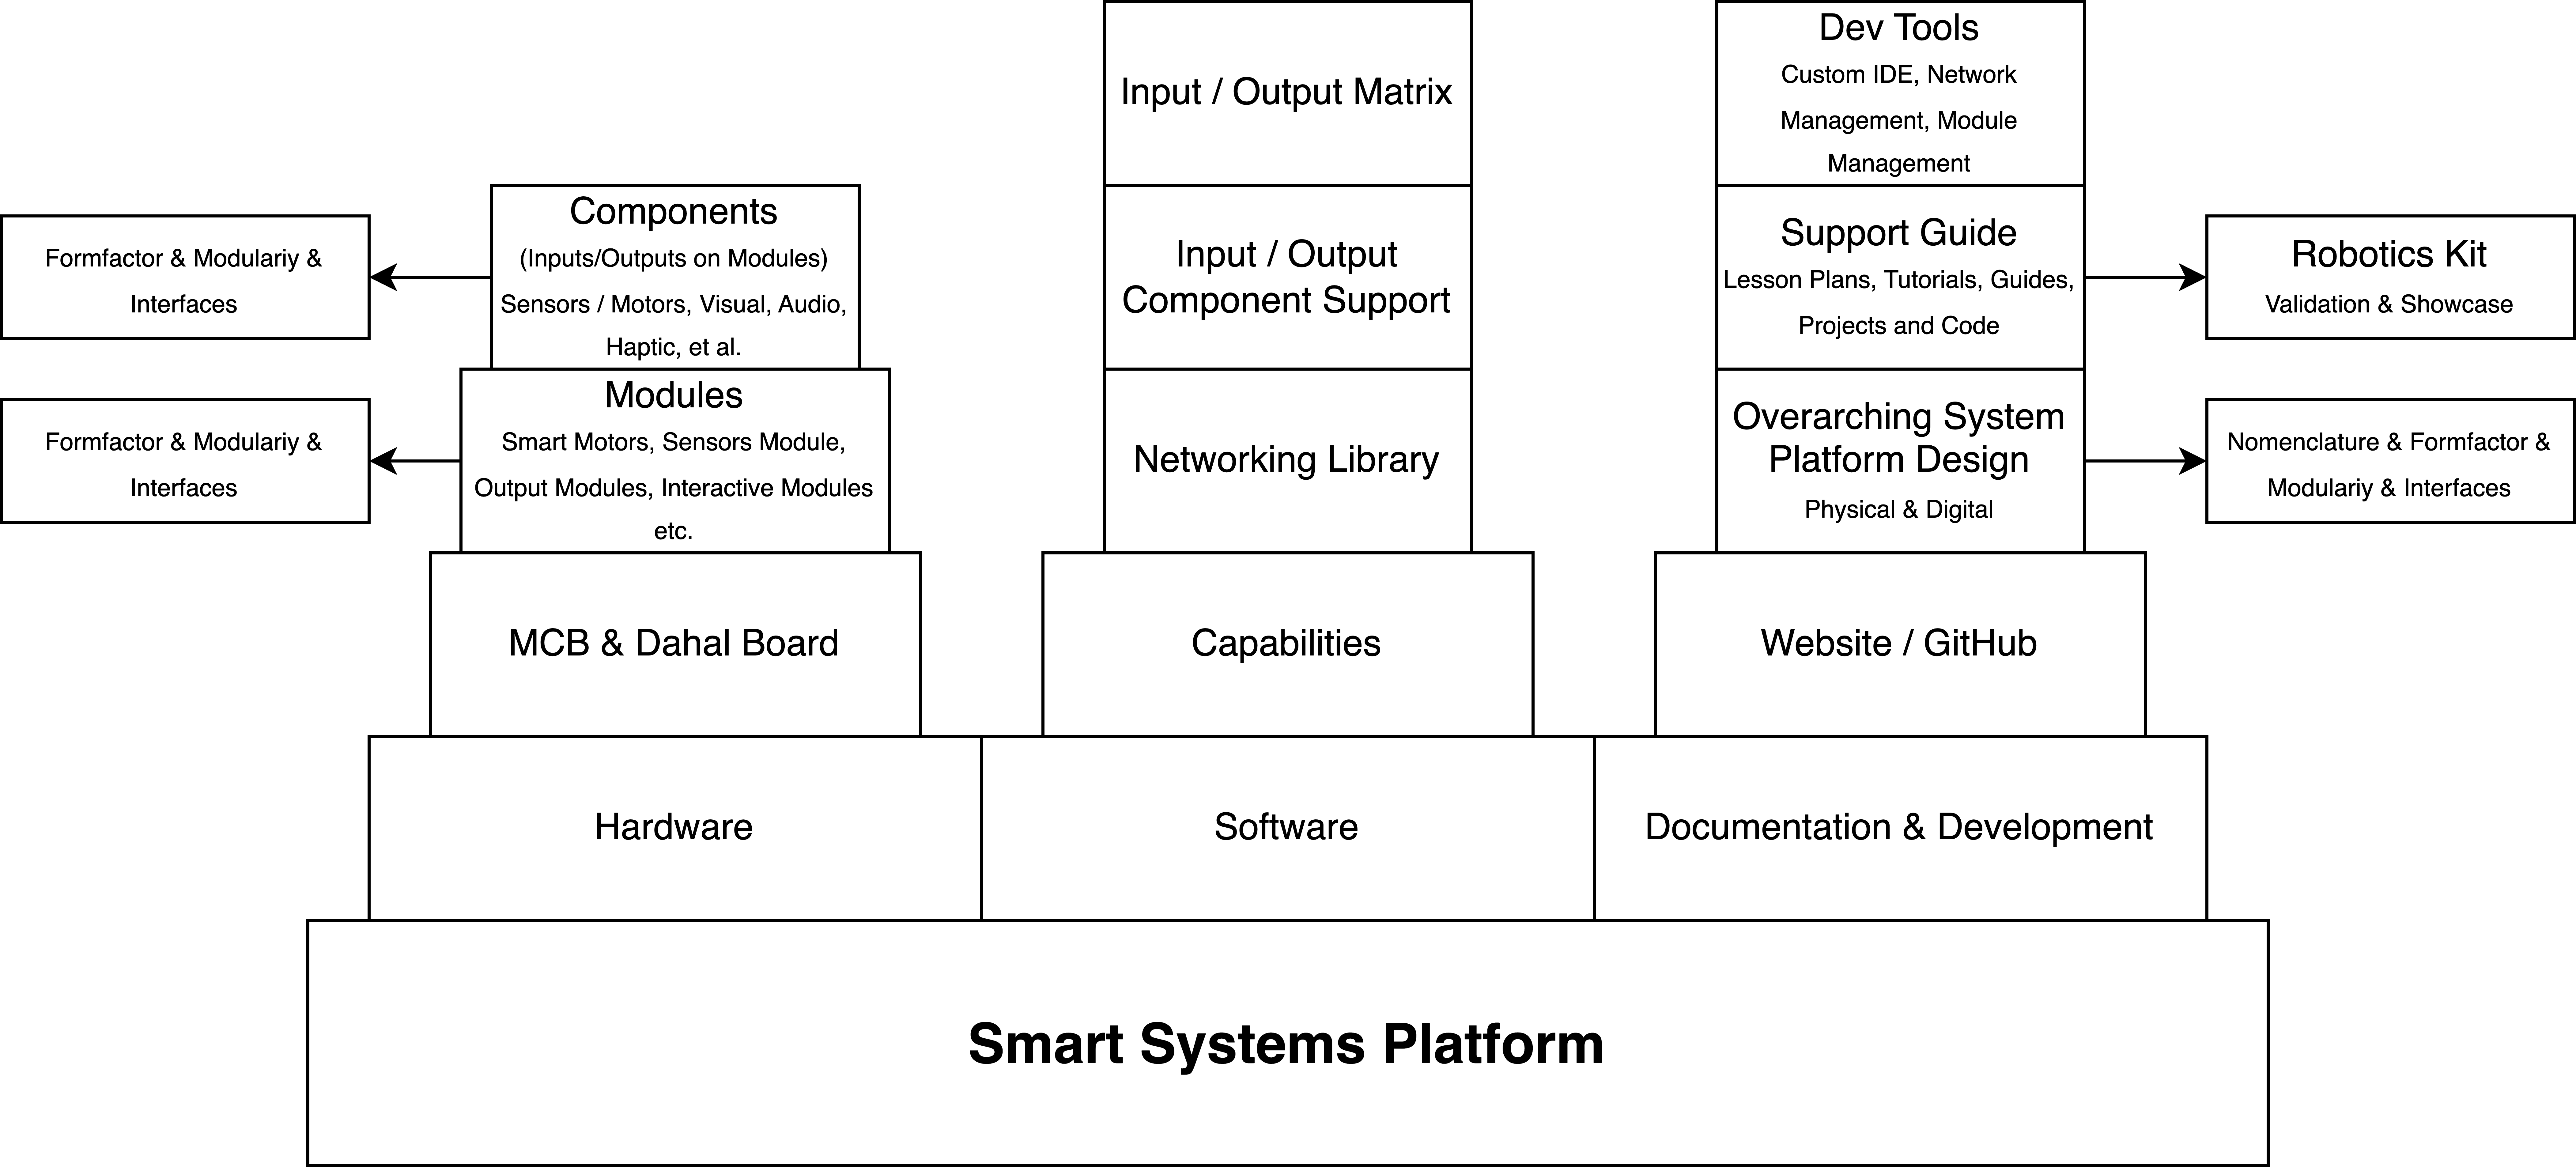
\includegraphics[width=\linewidth]{overleaf/images/Smart Systems Platform.drawio.png}
    \vspace{\ftspace}
    \caption{Platform Architecture}
    \label{fig:ssp_architecture}
\end{figure}

Put in the design and architecture of the platform,


and present the developed GitHub page, layout, website, guides and stuff and its capabilities

\section{\label{sec:res_capabilities}Smart System Platform} %reference to methods

\subsection{\label{sec:res_website}Website}

Website and quick start Guides

the website was to be tested with the Google for Developers PageSpeed Insights, which resulted in an overall score of 100 out of 100 for both mobile and desktop version of the webpage.

\subsection{\label{sec:res_tools}Development and Management Tools}

pyscript page, and perhaps mention the AI idea and other stuff

\subsubsection{\label{sec:res_ide}Integrated Development Environment}

Mention capabilities and design choices. 

\begin{figure}[H]
    \centering
    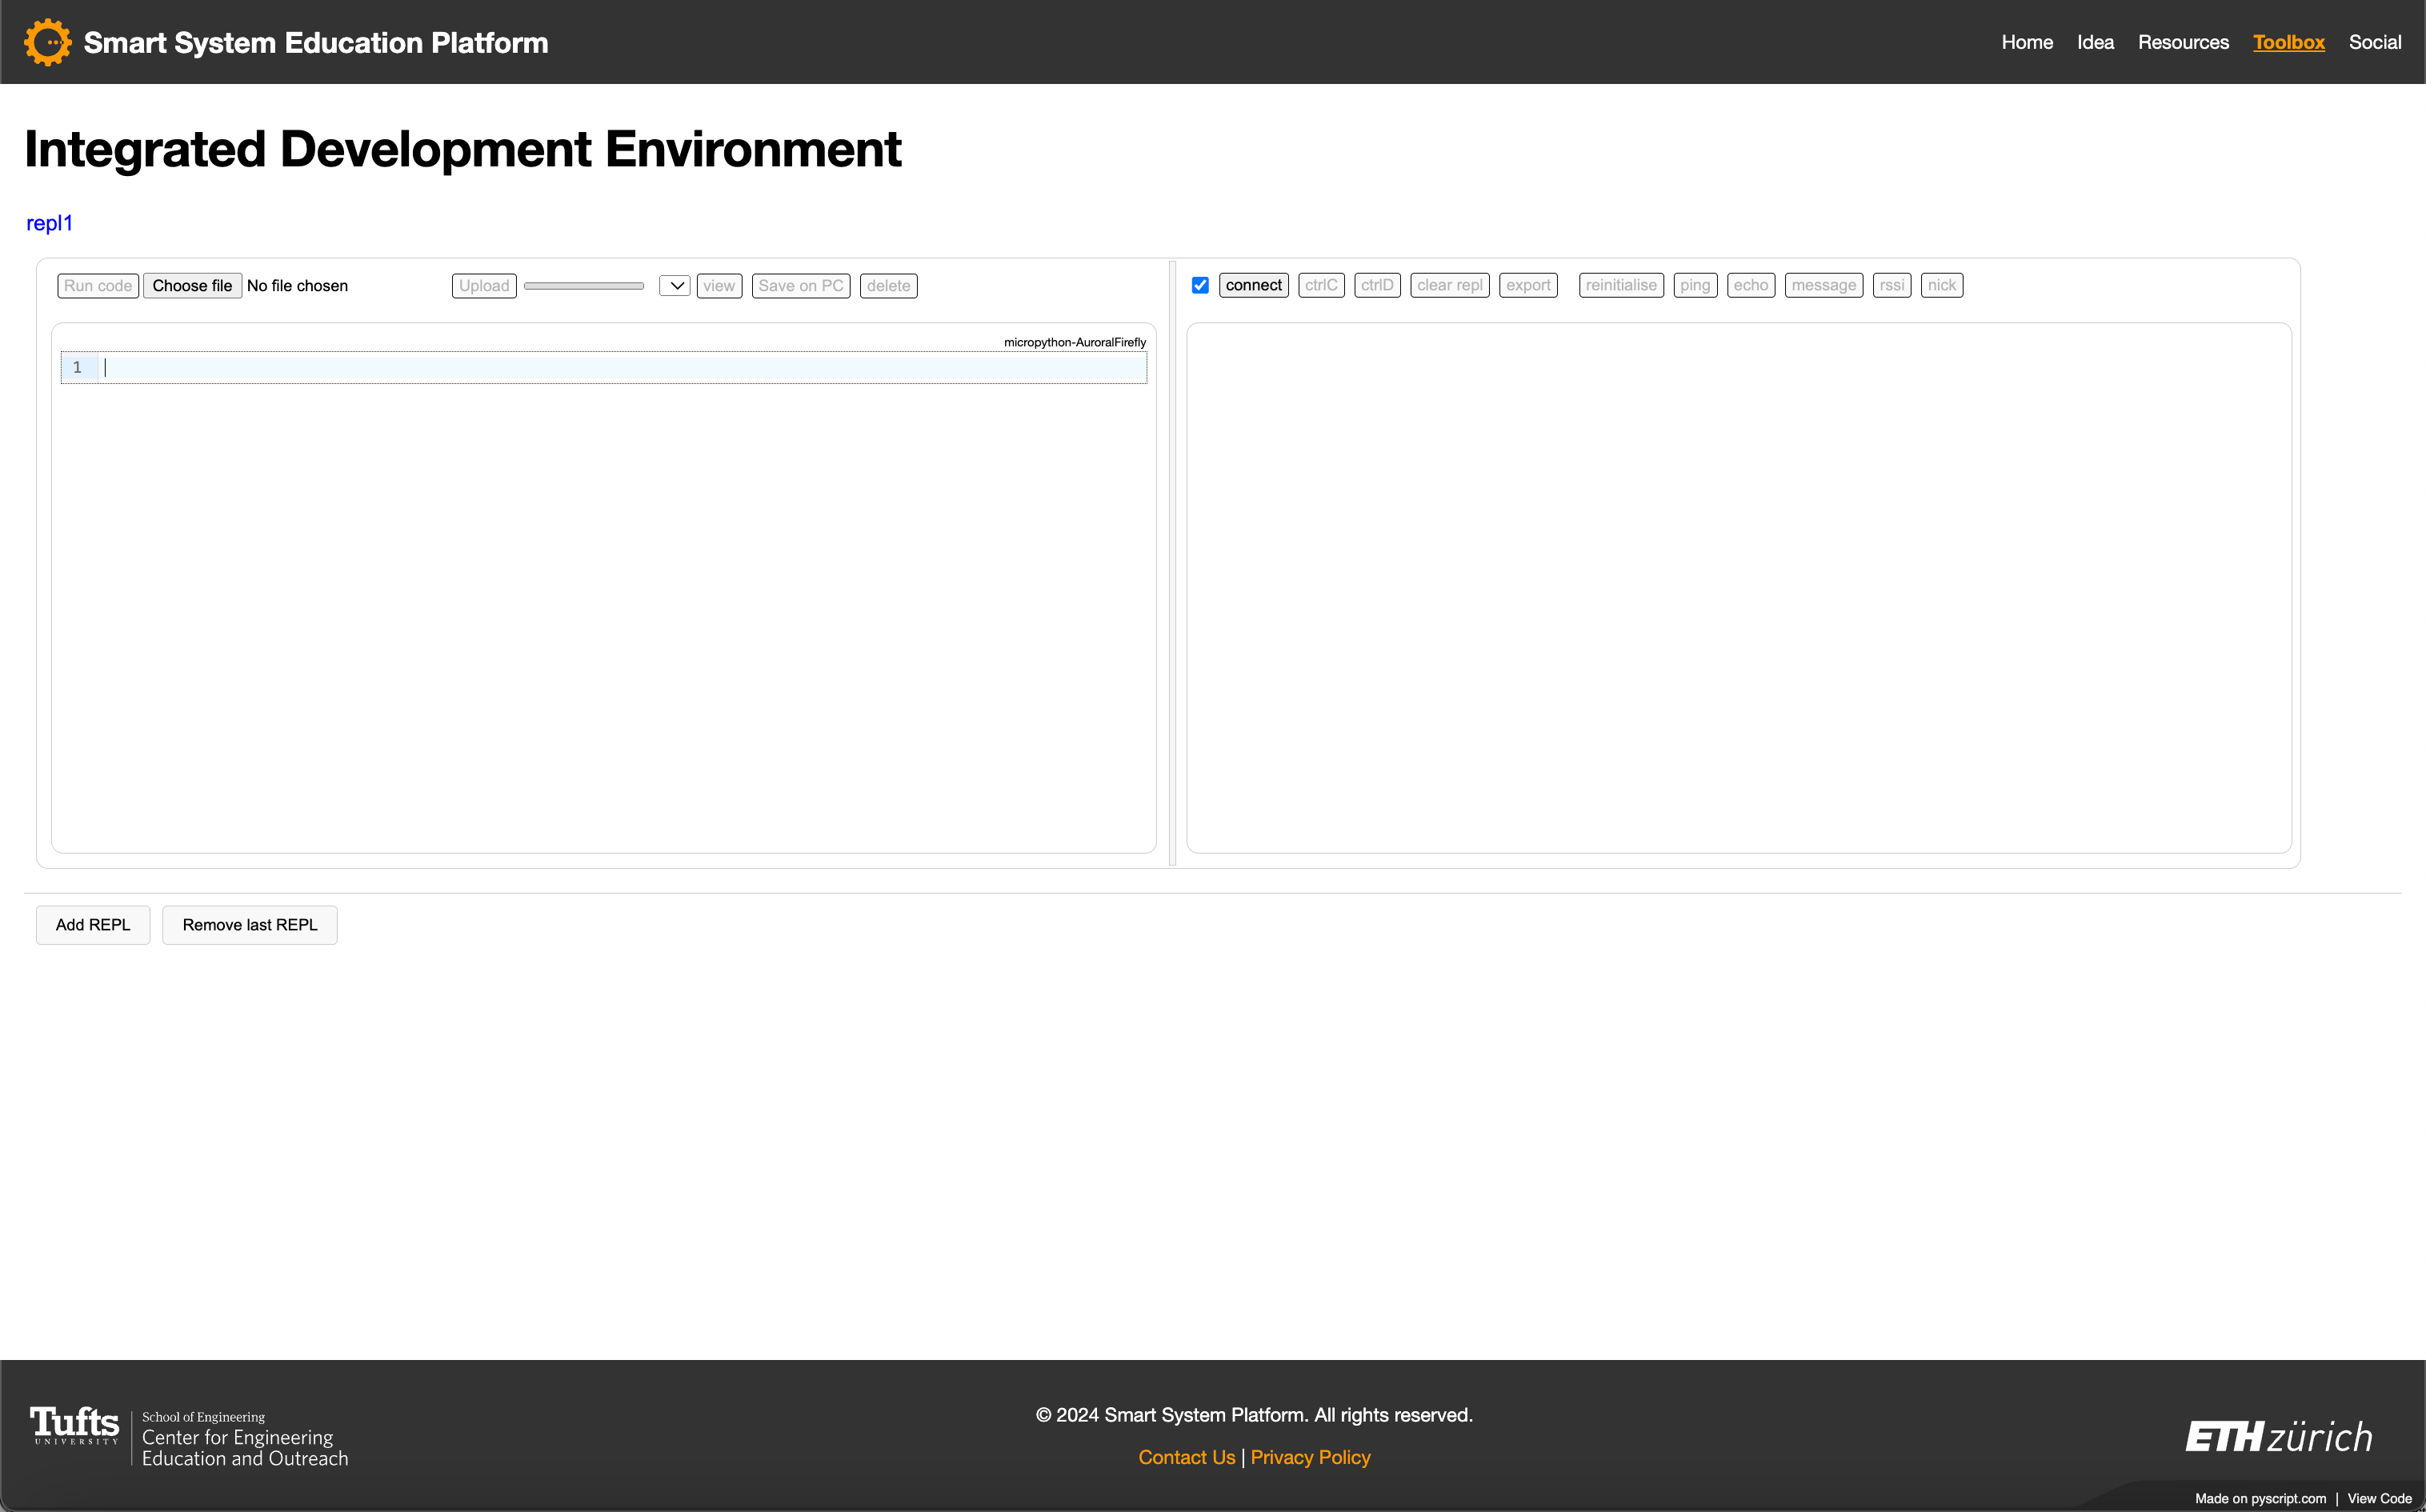
\includegraphics[width=\linewidth]{overleaf/images/ide_raw.png}
    \vspace{\ftspace}
    \caption{Custom SSP Web IDE}
    \vspace{\ftspace}
    \label{fig:ide_raw}
\end{figure}

\subsubsection{\label{sec:res_ai_code}AI Code Assistant}

Mention capabilities

\subsubsection{\label{sec:res_nmmct}Network Management and Module Configuration Tool}

Mention capabilities and design choices. 

\begin{figure}[H]
    \centering
    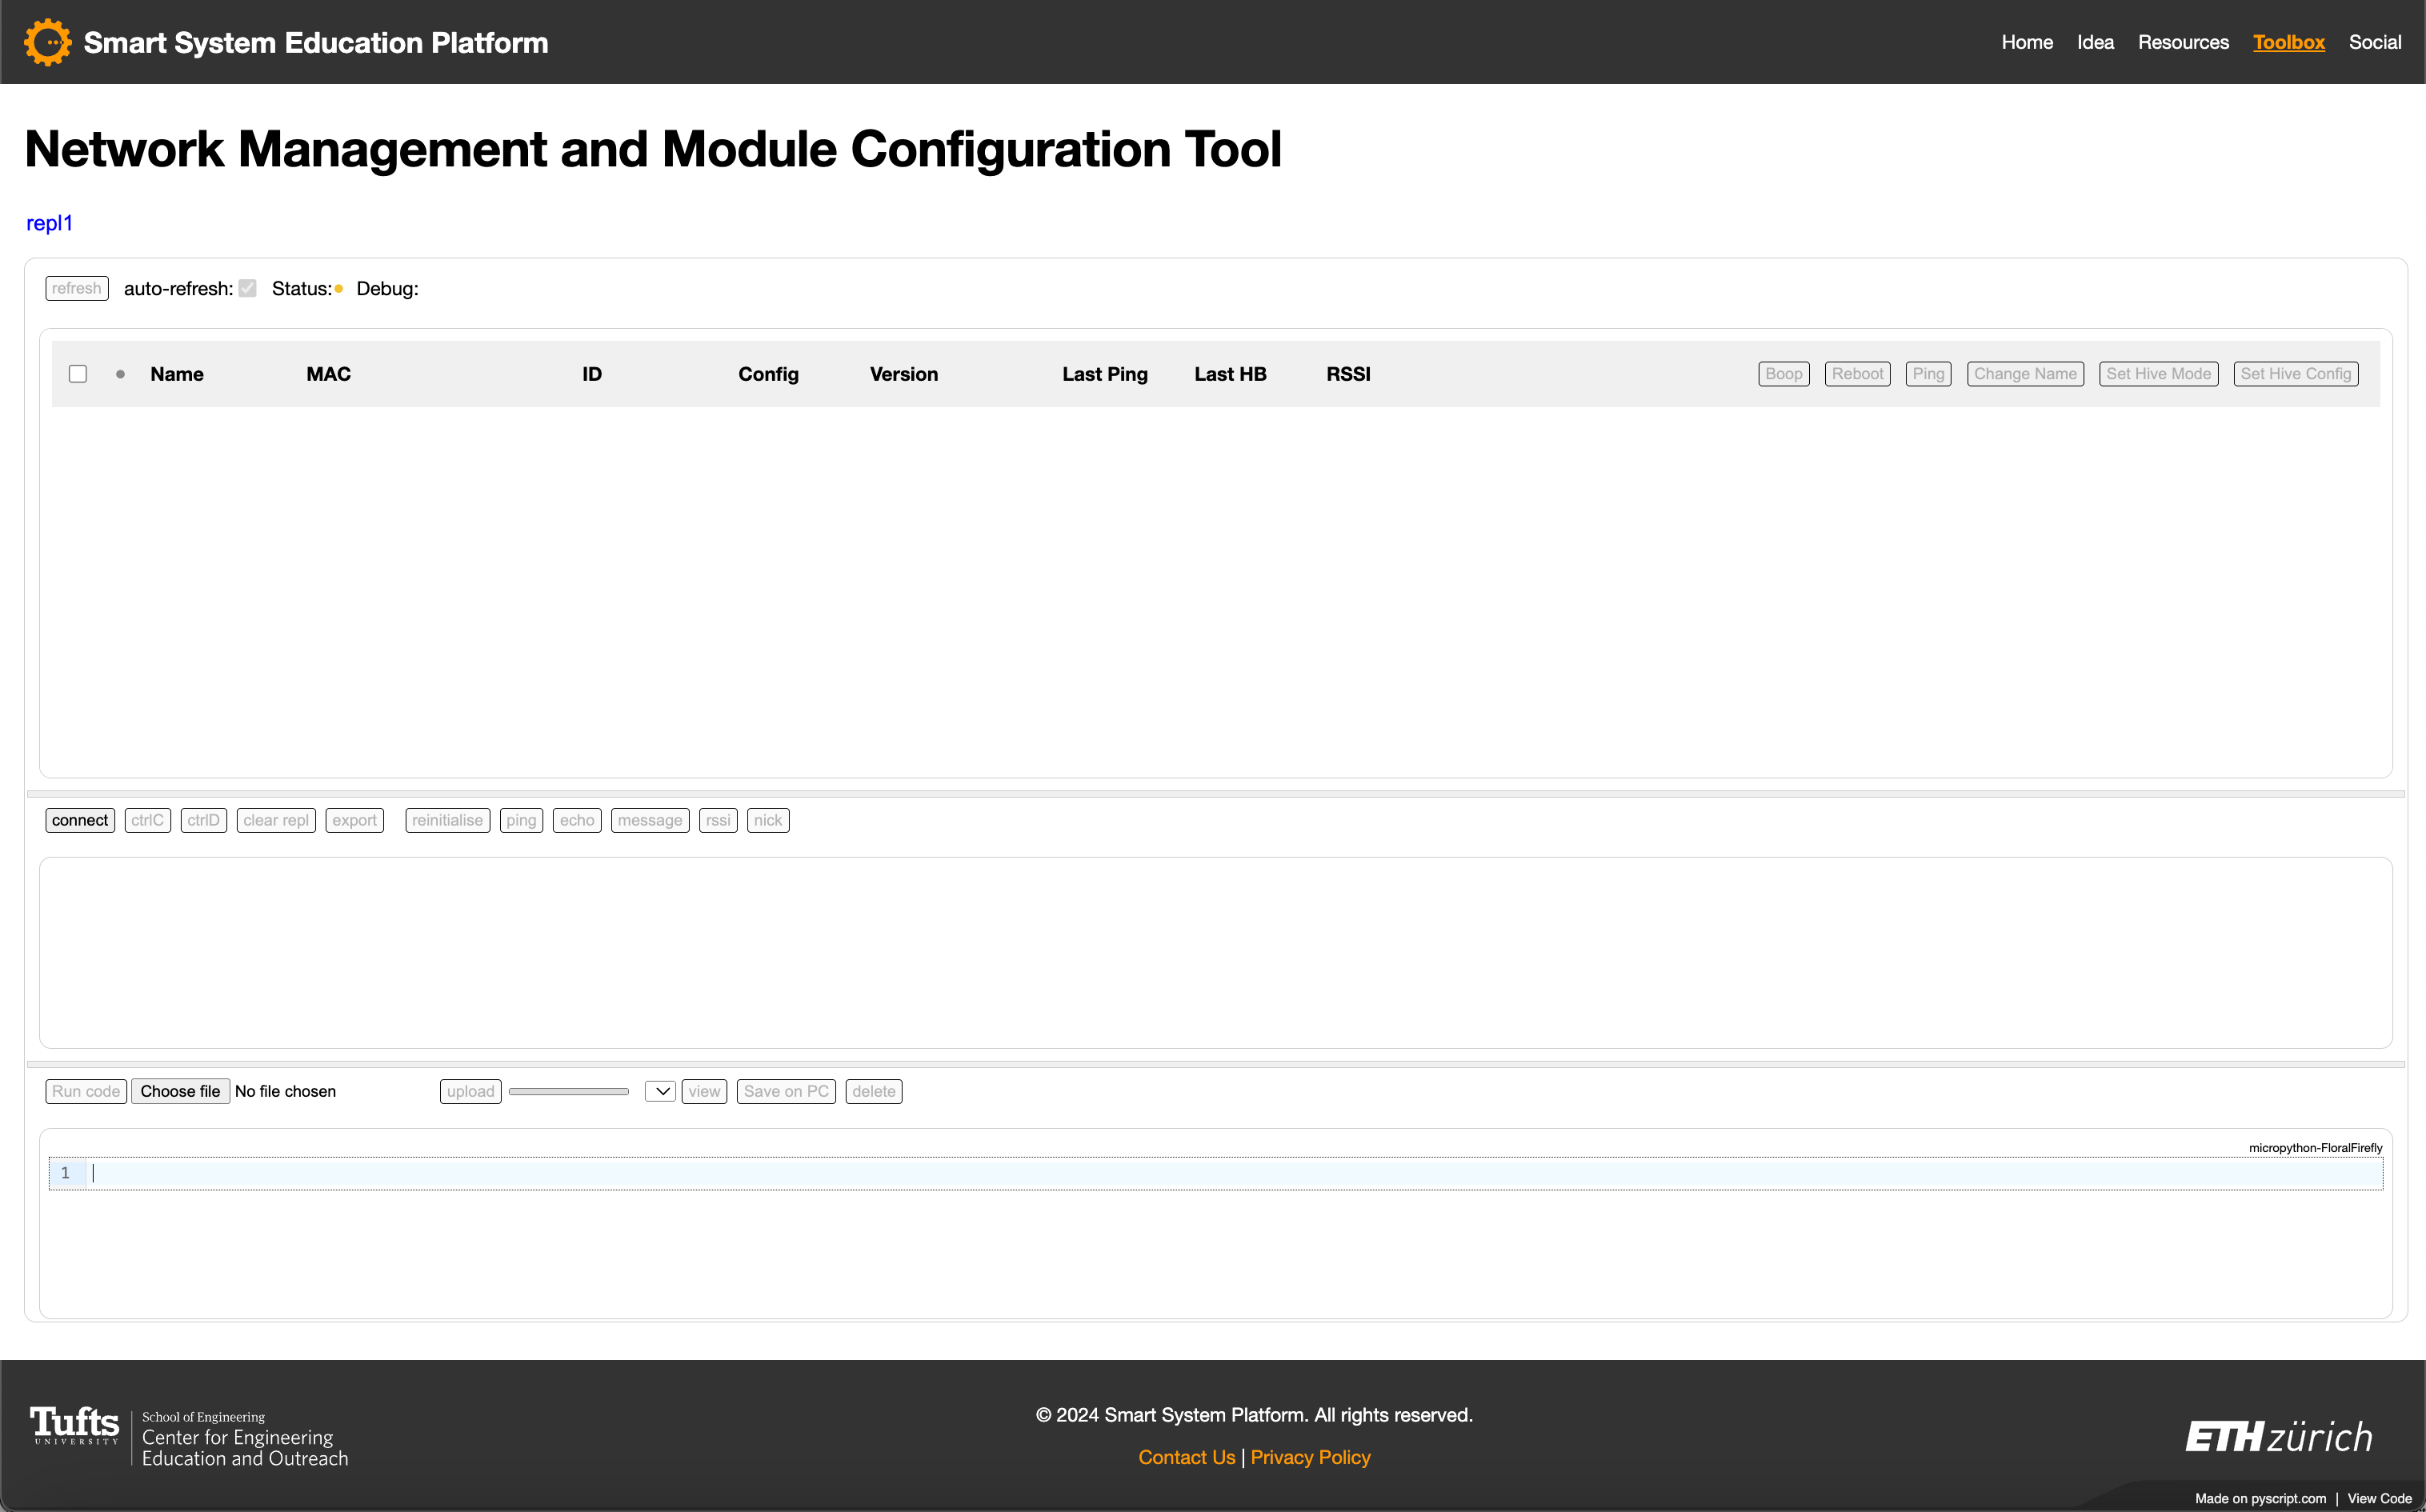
\includegraphics[width=\linewidth]{overleaf/images/nmmct_raw.png}
    \vspace{\ftspace}
    \caption{Network Management and Module Configuration Tool}
    \vspace{\ftspace}
    \label{fig:nmmct_raw}
\end{figure}

\subsubsection{\label{sec:res_ai_config}AI Module Configuration Assistant}

Give a quick mention of it.

\subsubsection{\label{sec:res_mmt}Module Management Tool}

Allows modules to be updated to the newest software. 

\begin{figure}[H]
    \centering
    
\includegraphics[width=0.5\linewidth]{overleaf/images/placeholder.png}
    \vspace{\ftspace}
    \caption{Module Management Tool}
    \vspace{\ftspace}
    \label{fig:mmt}
\end{figure}

\subsection{\label{sec:res_hardware}Hardware}

Module approach

Future board

etc.

in Figure \ref{fig:met_hardware}.

\subsection{\label{sec:res_software}Software}

main programs and stuff

different main codes for different modules, incl. configurable main code for various modules 


\section{\label{sec:res_validation}Validation}

\subsection{\label{sec:res_examplekit}Example Applications}
%ehhhhhhhhh, maybe present the three little programs I had written here

In a first step, interconnected Smart Motors, which use each others sensors as inputs were hard coded, using the Networking Library. 

Hive Modules: Explain how it works, directly configurable using the Network Management and Module Configuration Tool, without any coding required. 

\subsection{\label{sec:res_hackathon1}Hackathon 1}

Networking developed and idea gathering on how it could be used.

Result from the hackathon was that it was too complicated to get started, furthermore, the amount of messages sent was overwhelming since everybody was sending to everybody. Most people were not able to build anything useable. 

Main take-away of making it more approachable, include example code and a better guide. This has then lead to the development of development tools.

\subsection{\label{sec:res_hackathon2}Hackathon 2}

Test of development tools and application potential for educational or fun activities.

\subsection{\label{sec:res_honourablementions}Use in Other Projects}

mention playground project which made a lot of use of networking capability

Limitations?

\subsubsection{\label{sec:res_smartplayground}Smart Playground}

The Smart Playground Project has been the most prominent user of the Smart System Platform Networking Library. 

get feedback from them. Explain what they used networking for.

Certain battery and rssi angle test were directly influenced by anecdotal experience reports of using the Networking Library.

One of the reported issues, that they ran into is battery usage when using an ESP32C6, powering an audio output device, LED and using networking at the same time. Power supply in this case was provided by 3 AA batteries, though after 15 minutes the current had dropped too low with the device becoming stuck in a boot-loop.

Power consumption and use of multiple peripherals is something to consider for future development and use. 

The issue was specific to the Splat hardware, and likely due to the use of the batteries instead of LiPo batteries that were used in the Smart Motors. 

\subsubsection{\label{sec:res_me35}ME35}

The base networking module has been used by students for something.

How did they like it?

Limitation: Feedback is limited as only some students have used the library for their projects. Though from these students, feedback has been positive.